% !TeX spellcheck = en_GB
\documentclass[a4paper]{article}
%\documentclass[a4paper]{scrartcl}
\usepackage[utf8]{inputenc}
\usepackage[british]{babel}
\usepackage[backend=biber,sorting=none]{biblatex}
\addbibresource{bibfile.bib}
\usepackage{fullpage,amsmath,float,graphicx,parskip,fancyhdr,textcomp,csquotes,xcolor, geometry,gensymb}
\usepackage{subcaption,listings}
\setlength{\headheight}{12pt}
\setlength{\headsep}{25pt}
\usepackage[margin=10pt, font=small, labelfont=bf, labelsep=endash]{caption} %mooiere captions
\pagestyle{fancy}
\fancyhf{}
\fancyhead[L]{\bfseries\leftmark} %places section number and name in top left
\fancyhead[R]{\bfseries\thepage}%places pagenumber in top right
\usepackage[hidelinks]{hyperref}
\hypersetup{
	colorlinks,
	linkcolor={red!20!black},
	citecolor={blue!50!black},
	urlcolor={blue!80!black}	}
\lstset{ 
	commentstyle=\color{olive},    % comment style
	keywordstyle=\color{blue},       % keyword style
	numbers=left,                 
	stringstyle=\color{brown},     % string literal style
	tabsize=2,	                   % sets default tabsize to 2 spaces
}
\title{\textbf{Analysis of the Ising model} \\\large{Exercise 2.3 and 2.4, Modelling and Simulation}}
\author{Jim Carstens (5558816)}
\date{\today \\ 
\includegraphics[scale=0.4]{uulogo.pdf}}

\begin{document}
\maketitle
\hrulefill
\tableofcontents
\hrulefill
%%%%%%%%%%%%%%%%%%%%%%%%%%%%%%%%%%%%%%%%
\section*{Introduction}
In this report, the Ising model will be investigated using both the Metropolis algorithm and the Wolff algorithm. The Ising model is an important mathematical model which can be used to describe physical systems such as magnets and grids of correlated spins and there are even applications in neuroscience. 

For a two-dimensional Ising model, the average magnetisation, energy, heat capacity, magnetic susceptibility and autocorrelation functions are investigated using a Monte Carlo model. Two different algorithms for implementing the Ising model are tested and compared: the Metropolis algorithm and the Wolff algorithm.

%%%%%%%%%%%%%%%%%%%%%%%%%%%%%%%%%%%%%%%%
\section{Theory}  \label{sec:c}
The Ising model describes a system of correlated spin states in a lattice. This correlation is given by the Hamiltonian of the system:
\begin{equation} \label{eq:ham}
	H=-J\sum_{\left<ij\right>}s_i s_j -B\sum_{i}s_i.
\end{equation}
In this equation, the first sum goes over $\left<ij\right>$, which means the nearest neighbours $j$ of particle $i$, $J$ is the alignment energy and $B$ is the strength of an external magnetic field. Spins $s_i$ can take on a value of either $-1$ or $+1$. By choosing $J$ to be positive, energy is lowered by aligning spins, resulting in ferromagnetic behaviour. On the contrary, choosing $J$ to be negative causes the energy to be lowered by anti-aligning spins. This results in anti-ferromagnetic behaviour. In this report positive $J$ is considered. Moreover, a model with no external field is examined, so $B = 0$. For the phenomena investigated here an external field is not necessary. However, adding it to the model would not be a complicated undertaking.

One can look at many different dimensionalities for the Ising model. The one-dimensional model was solved exactly in 1925 by Ising \cite{Ising:1925em}. In 1944, Onsager arrived at a mathematical solution for the 2D-model without an external magnetic field \cite{1944PhRv...65..117O}. No solution has been found for the 3D-model so far, nor for higher dimensions. Numerically, as well as analytically with the right approximations however, many research as been done and much is known about the Ising model in these conditions. In this report, the two-dimensional Ising model is chosen to investigate.

An interesing property of this 2D-model is the presence of a phase transition, which the 1D-version does not have. The phase transition, which happens at the critical temperature $T_C$ divides the behaviour of the system in two regimes. Below $T_C$, the thermal fluctuations are not so large and spontaneous magnetisation occurs. Here the system is ferromagnetic. Above $T_C$, the thermal fluctuations are large enough to destroy the magnetisation of the system.

Several properties are interesting to measure. The mean magnetisation of the system is simply a sum of all the spins in the system:
\begin{equation} \label{eq:M}
	\left< M \right> = \left< \sum_{i} s_i \right>.
\end{equation}

The energy of the system can be calculated using the Hamiltonian of \autoref{eq:ham}. For both quantities it is also interesting to divide them by the amount of lattice points $N$. In the case of the magnetisation, this gives $\left< m\right>=\left< M \right>/N$. From these quantities, two more properties of the system can be calculated, the heat capacity 
\begin{equation}
	c_S = \frac{\beta^2}{N} \left( \left<E^2\right> -\left<E\right>^2\right), 
\end{equation}
and the magnetic susceptibility 
\begin{equation}
 \chi_m = \beta N \left( \left<M^2\right> -\left<M\right>^2\right),
\end{equation}

where $\beta=\frac{1}{k_B T}$. In this report, $k_B$ is taken to be 1.

The autocorrelation of a certain quantity can be calculated as follows \cite{newman1999monte}:
\begin{equation}
C_M(t)= \frac{1}{t_max-t} \left( \sum_{t'=0}^{t_{max}-t} M(t')\times M(t'+t)- \sum_{t'=0}^{t_{max}-t} M(t') \times \sum_{t'=0}^{t_{max}-t} M(t'+t) \right).
\end{equation}

In this formula specifically $C_M$, the magnetic autocorrelation function is given. By switching $M$ for another quantity, other autocorrelation functions can be computed.

\section{Simulation}
For the simulation, a program is made in C\texttt{++} that generates a two-dimensional square lattice of width $L$ with total system size $N=L\times L$. This lattice is represented by an array containing \texttt{int} values of $\pm1$, where the positive value arbitrarily corresponds to spin-up, and the negative value to spin-down. The system can be initialised either to a temperature $T=0$, where all spins point in the same direction, or to $T=\infty$, where all spins are randomly chosen. For generating random numbers the generator \texttt{std::mt19937} is used with as seed the current time \texttt{std::chrono::steady\_clock::now().time\_since\_epoch().count()}. This provides quick, highly random numbers.

Since the lattice is not of infinite size (this would require infinite computational power), periodic boundary conditions are used.  This means that each site at the edge of the lattice has the other side of the lattice as its neighbours, as can be seen in \autoref{fig:pc}.
\begin{figure}[h]
	\centering
	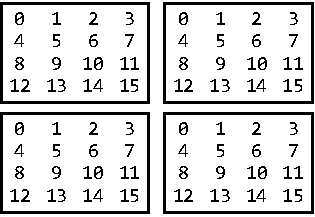
\includegraphics[width=0.3\textwidth]{latimage.pdf}
	\caption{Periodic boundary conditions}
	\label{fig:pc}
\end{figure}
Another approach that can be used are helical boundary conditions, which are much faster to compute. There, the 2D-lattice is reduced to a 1D-lattice that is wrapped around itself. The neighbours can be calculated using arithmetic. A way to imagine this is by thinking about a film roll wrapped around a cylinder, where aligned frames are neighbours.

In this report, periodic boundary conditions are used because it allows for legible code. Moreover, a variant on the normal Ising model is considered here. Normally the nearest neighbours $\left<ij\right>$ of a spin that are considered are the four neighbours left, right, up and down. Here however, also the corner neighbours are considered. This brings the amount of neighbours to 8. For example, for site 10, the neighbours are $(5,6,7,9,11,13,14,15)$.

When running the program, first, the system is started out at $T=0$, or $T=\infty$ and allowed to equilibrate to the composition correspondign to the actual temperature that is set. Then, for many Monte Carlo steps, the spins are flipped according to an algorithm, the various observables are measure using equations \ref{eq:ham} and \ref{eq:M}. Then, the temperature can be changed and the previous is repeated. 
For each measurement of the energy and the magnetisation, 100 samples are taken at intervals of 100, after the system has been at a certain temperature for 1000 Monte Carlo steps. Later, this will prove to be sensible.

\section{Metropolis algorithm}
\subsection{Method}
The Metropolis algorithm works by flipping single flips and accepting a move according to the acceptance rule. This is also called single flip dynamics. 
This acceptance rule is as follows:
\begin{equation}
A(\mu \rightarrow\nu) = \begin{cases}
e^{\beta \Delta E} \quad \text{if} \Delta E>0 \\
1 \quad \text{if} \Delta \leq 0
\end{cases}
\end{equation}
For each Monte Carlo move, $N$ single flips are attempted. Thus, on average, each site will be visited during each move. Because a single flip can be undone with an equal chance, this algorithm preserves ergodicity.

The measurements are performed by at the beginning of the simulation computing the energy and magnetisation for the whole system, and from then on adding the difference, to save computation time. Here 
\begin{equation}
\Delta E = 2J s_k^{\mu} \sum_{\left<ij\right>} s_i^{\mu},
\end{equation}
and
\begin{equation}
\Delta M = 2 s_k^{v}
\end{equation}
are used.
The other quantities can be calculated from the former. The magnetization autocorrelation function is calculated after the simulation, by looking at 1000 consecutive measurements for the magnetisation right after setting the temperature. Then, in Wolfram Mathematica, the following formula is used:
\begin{lstlisting}
	mac = Table[1/(tmax - t)*Sum[mdat[[t2]]*mdat[[t2 + t]], {t2, 1, tmax - t}] - 
	Sum[mdat[[t2]], {t2, 1, tmax - t}] *
	Sum[mdat[[t2 + t]], {t2, 1, tmax - t}], {t, 1, tmax - 1}];
\end{lstlisting}

The acceptance values are pre-calculated and stored in an acceptance array after setting the temperature, to avoid needing to calculate these exponents every spin swap step.

The code that was used can be seen in \autoref{sec:met}.

\subsection{Results}
In \autoref{fig:wolff}, the results of calculating various quantities along a range of temperatures are displayed, for the energy and the magnetisation with errors. However, these errors are so small that they are not visible. It can be seen that at low temperatures, the system is fully magnetised, corresponding to the lowest possible energy $E=8J/\text{spin}$, which is the amount of neighbours a spin has. Upon increasing temperature, not much happens, until the critical temperature is reached. There, the magnetisation drops to zero, and the enery also goes to zero. The thermal fluctuations overpowerd the paramagnetic tendencies of the material. In the program, this is a result from the fact that at high temperature, many moves that rise the energy are also accepted.
\begin{figure}[H]
	\centering
	\begin{subfigure}[b]{0.4\textwidth}
		\centering
		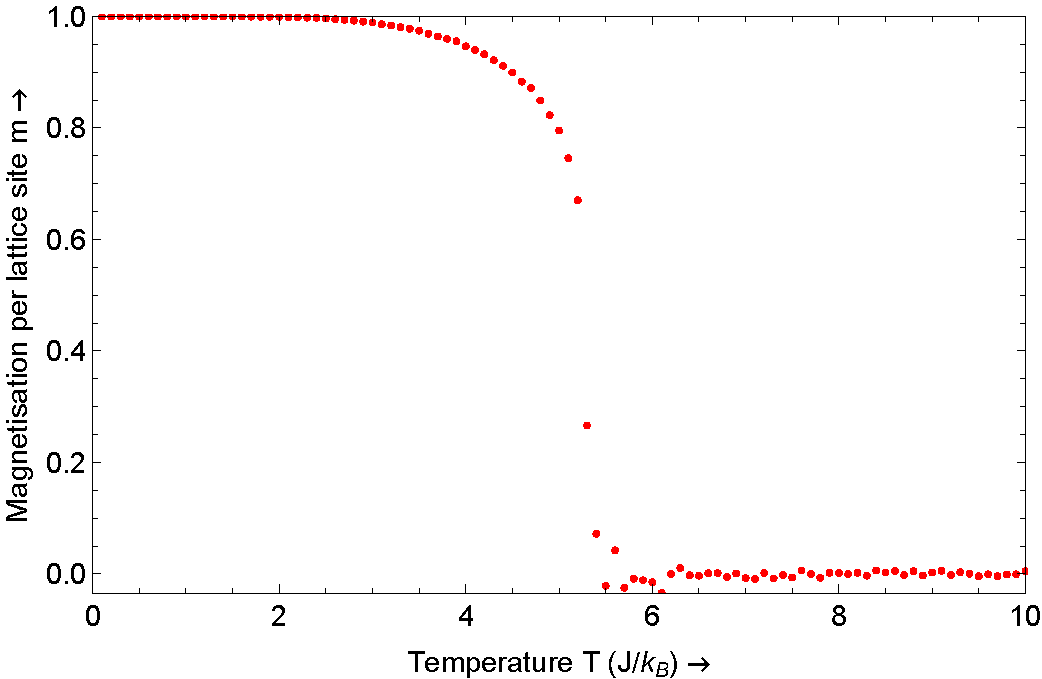
\includegraphics[width=\textwidth]{magplot.pdf}
		\caption{ Magnetisation over temperature}
	\end{subfigure}%
	\begin{subfigure}[b]{0.4\textwidth}
		\centering
		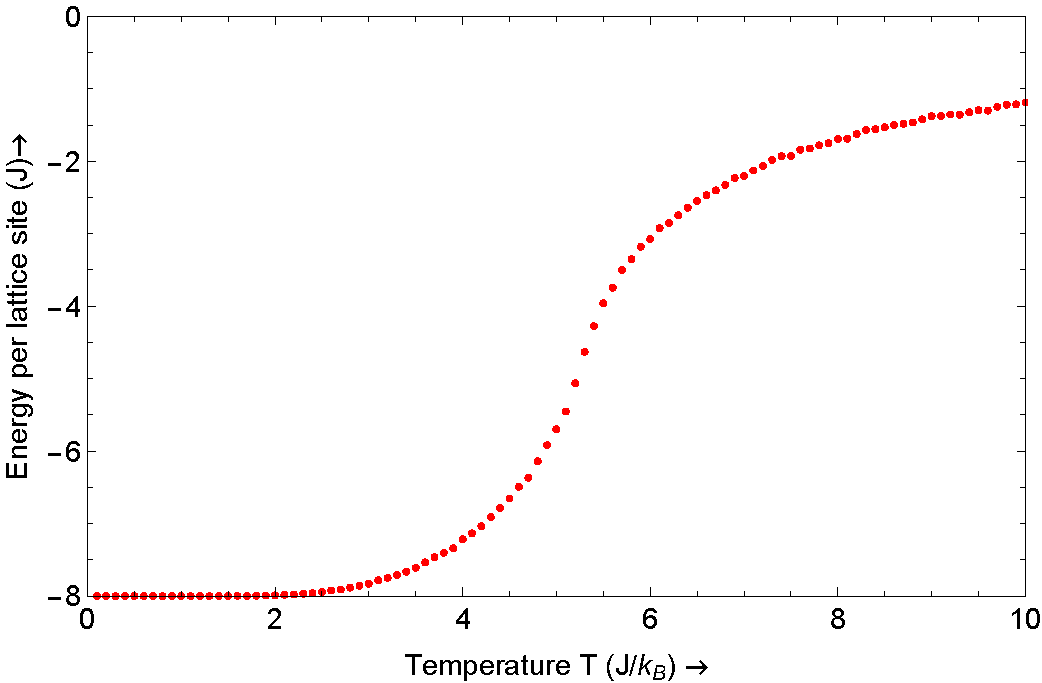
\includegraphics[width=\textwidth]{eplot.pdf}
		\caption{Energy over temperature}
	\end{subfigure}%
	\\
	\begin{subfigure}[b]{0.4\textwidth}   
		\centering
		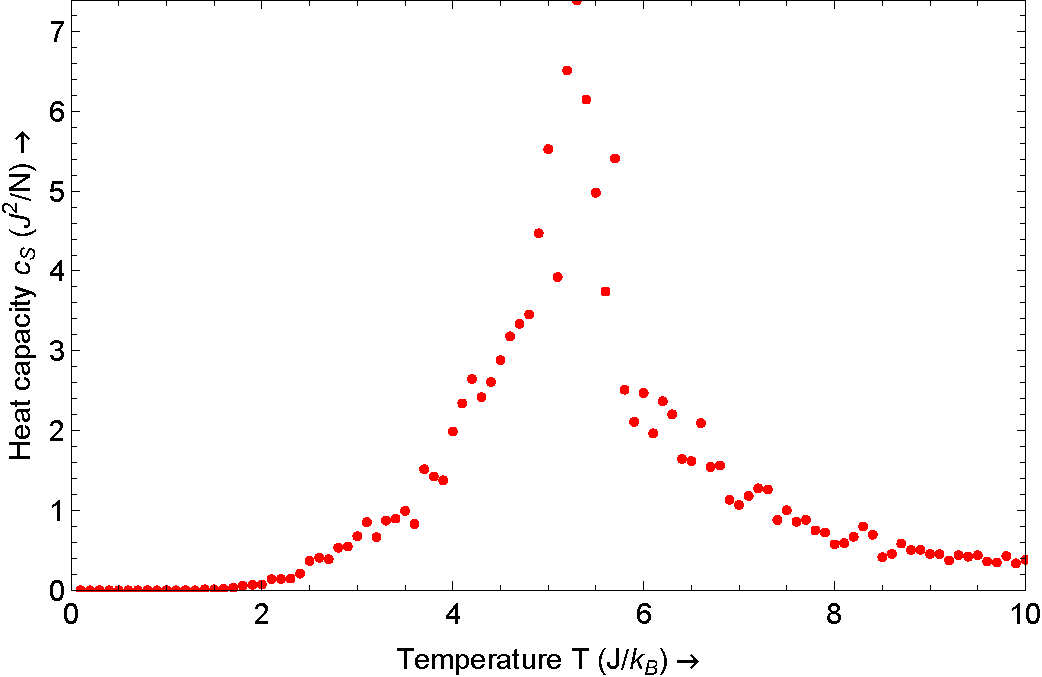
\includegraphics[width=\textwidth]{hcplot.pdf}
		\caption{Heat capacity over temperature}
	\end{subfigure}%
	\begin{subfigure}[b]{0.4\textwidth}
		\centering
		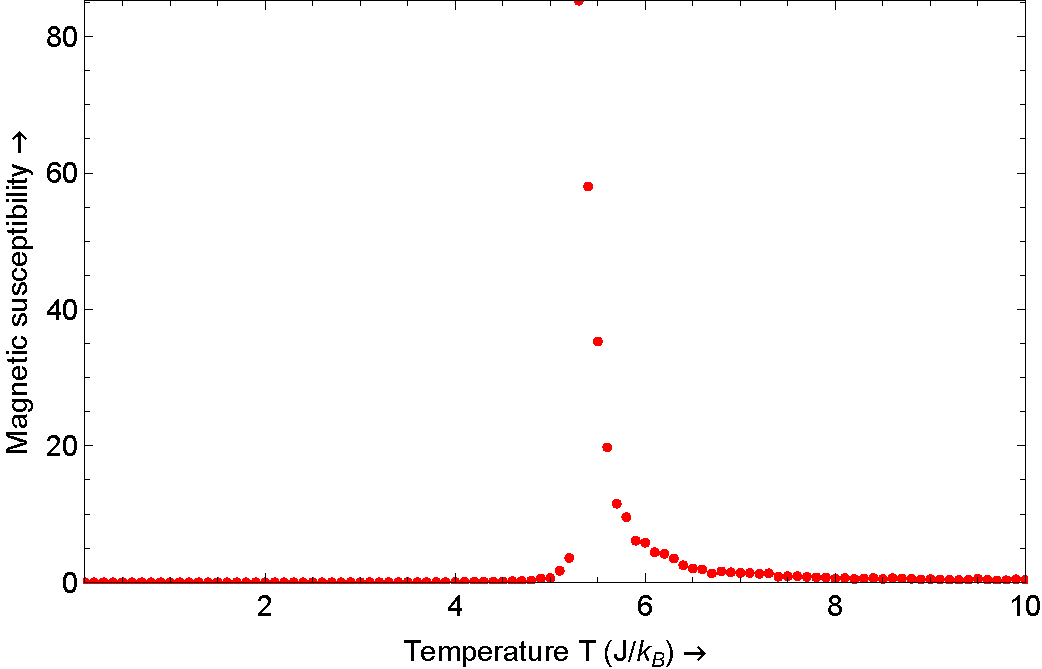
\includegraphics[width=\textwidth]{magsusplot.pdf}
		\caption{Magnetic susceptibility over $T$}
	\end{subfigure}
	\caption{Plots of the magnetisation(including errors), energy (including errors), heat capacity and magnetic susceptibility against temperature. All values are per lattice site for clarity.}
	\label{fig:metropolis}
\end{figure}

The heat capacity and the magnetic susceptibility obtain a very high value around the critical temperature. The critical temperature is estimated for this system to be $T_C=5.3 J$. No theoretical background on the eight-neighbour Ising model was found to compare this value to.

In \autoref{fig:macM}, it can be seen that the magnetic autocorrelation is very stable before $T_C$ and much less after $T_C$.

\begin{figure}[h]
	\centering
	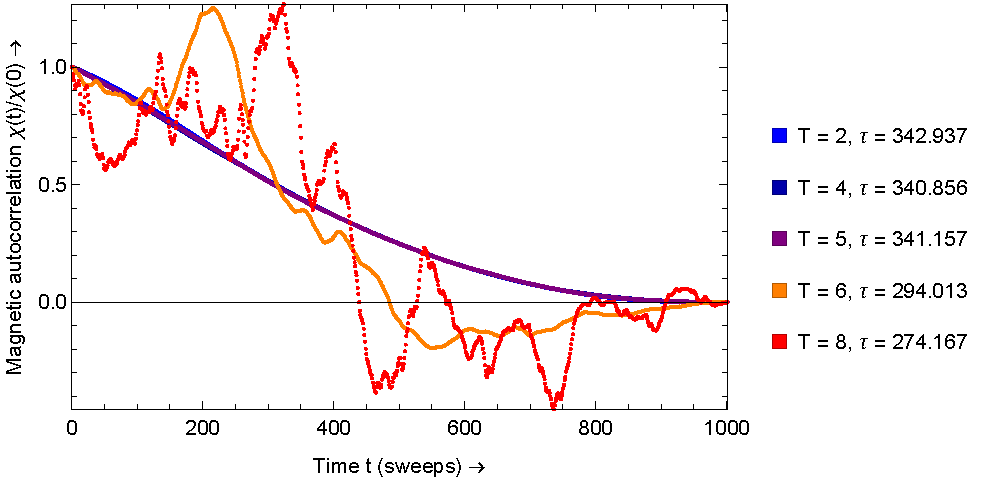
\includegraphics[width=0.6\textwidth]{macimage.pdf}
	\caption{The magnetic autocorrelation function $C_M$ calculated for various temperature. The correlation time is displayed in the legend.}
	\label{fig:macM}
\end{figure}

%%%%%%%%%%%%%%%%%%%%%%%%%%%%%%%%%%%%%%%%%%%%%%%%%%%%%%%%%%
\section{Wolff algorithm}
\subsection{Method}
Wolff's algorithm is used to overcome the long correlation times of the Metropolis algorithm around the critical point. It works by finding clusters of same spins and flipping them all according to a certain probability. Spins are added to the cluster according to the following probability
\begin{equation}
P_{add} = 1-e^{-2\beta J}.
\end{equation}
The code that was used can be seen in \autoref{sec:wolf}.

\subsection{Results}
In \autoref{fig:wolff} the results for using the Wolff algorithm can be seen. In general, all results are rather similar to the results of the Metropolis algorithm. The difference is that the focus is more made on the region of the phase transition. Also, for the magnetic susceptibility, the divergence of the peak at $T_C$ is less extreme with the Wolff algorithm than with the Metropolis algorithm. The value for the critical temperature still seems to be $T_C=5.3 J$.
\begin{figure}[H]
	\centering
	\begin{subfigure}[b]{0.4\textwidth}
		\centering
		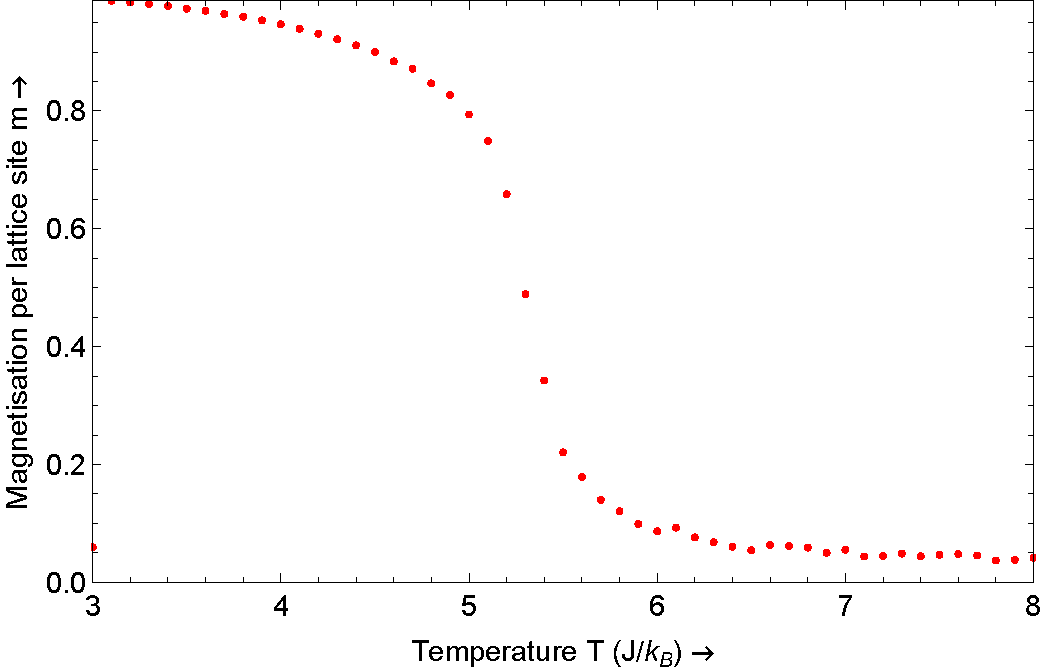
\includegraphics[width=\textwidth]{magplotW.pdf}
		\caption{ Magnetisation over temperature}
	\end{subfigure}%
	\begin{subfigure}[b]{0.4\textwidth}
		\centering
		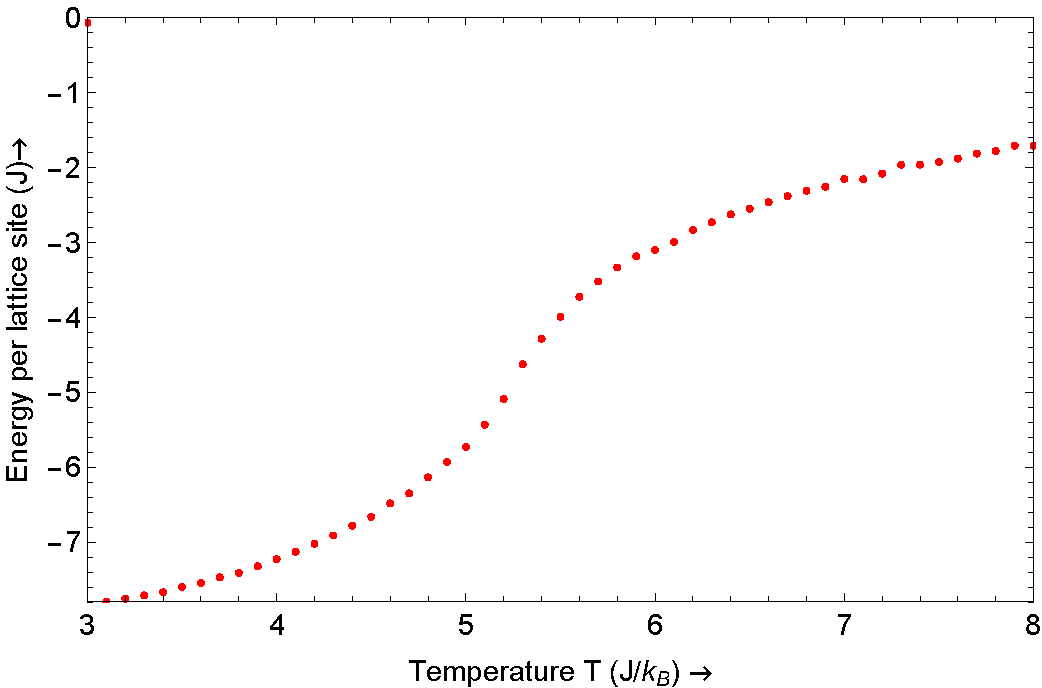
\includegraphics[width=\textwidth]{eplotW.pdf}
		\caption{Energy over temperature}
	\end{subfigure}%
	\\
	\begin{subfigure}[b]{0.4\textwidth}   
		\centering
		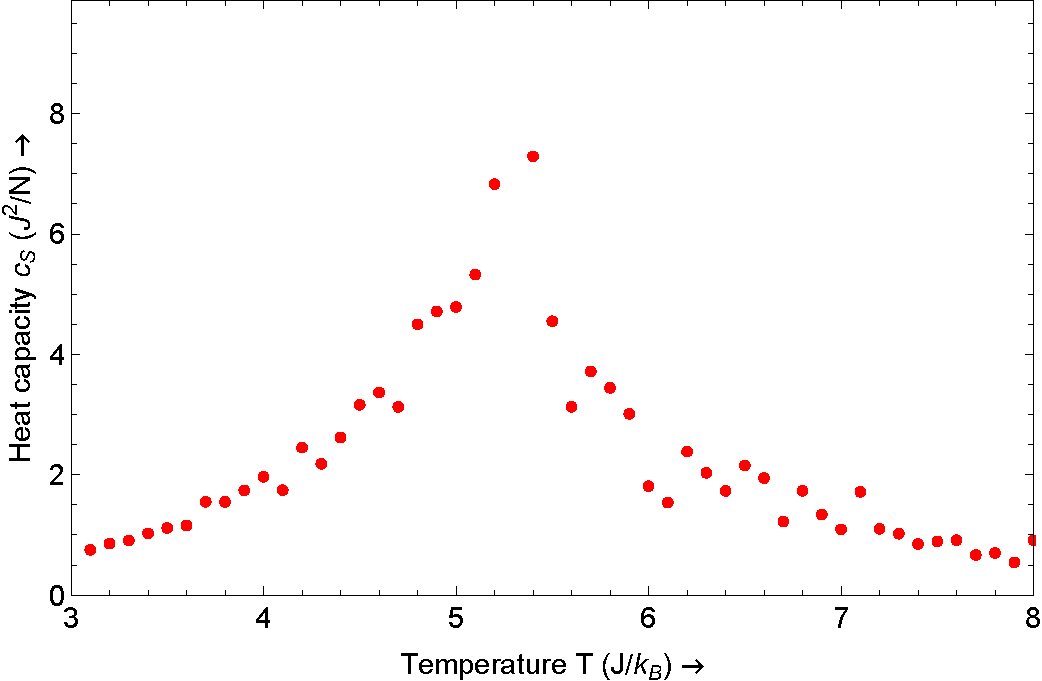
\includegraphics[width=\textwidth]{hcplotW.pdf}
		\caption{Heat capacity over temperature}
	\end{subfigure}%
	\begin{subfigure}[b]{0.4\textwidth}
		\centering
		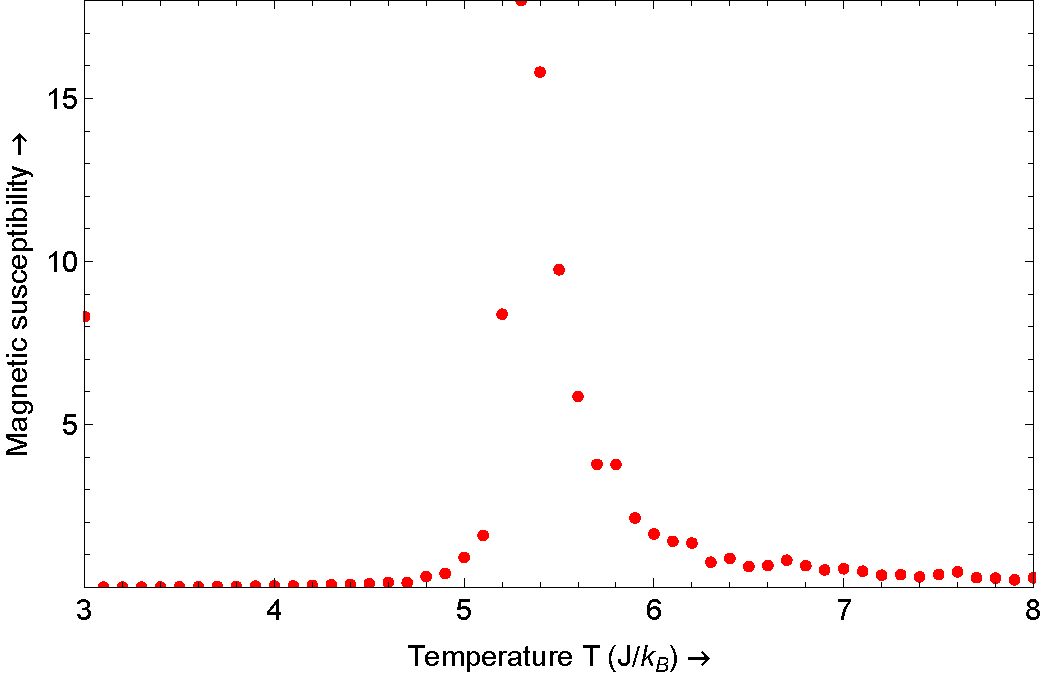
\includegraphics[width=\textwidth]{magsusplotW.pdf}
		\caption{Magnetic susceptibility over $T$}
	\end{subfigure}
	\caption{Plots of the magnetisation(including errors), energy (including errors), heat capacity and magnetic susceptibility against temperature. All values are per lattice site for clarity.}
	\label{fig:wolff}
\end{figure}

There is however a clear difference at the autocorrelation function. As can be seen in \autoref{fig:eac}, the autocorrelation function remains neat across all temperatures, even very close to the critical temperature. A qualitative observation is that after the critical temperature, the algorithm runs very fast. This is probably because there is so much thermal nosie that no big clusters can be formed.

\begin{figure}[h]
	\centering
	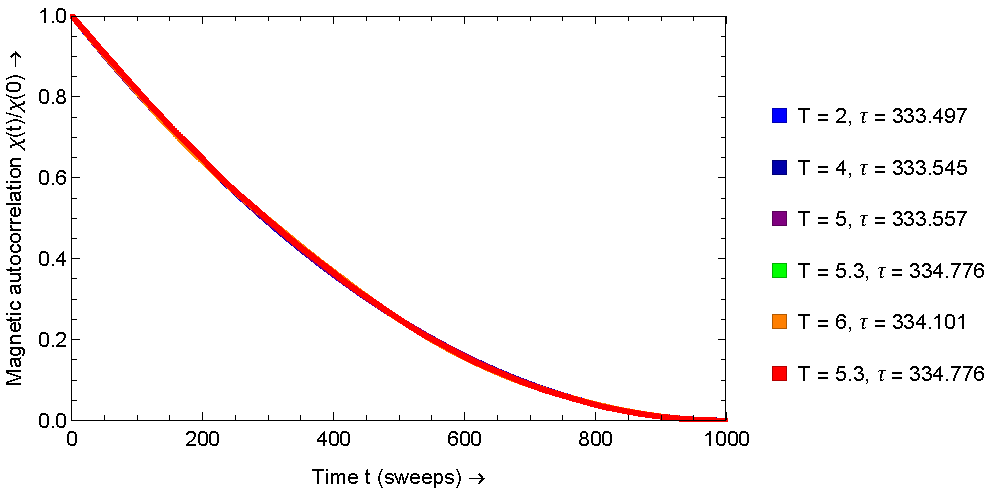
\includegraphics[width=0.6\textwidth]{macimageW.pdf}
	\caption{The energy autocorrelation function $C_E$ calculated for various temperature. The correlation time is displayed in the legend.}
	\label{fig:eac}
\end{figure}


\section{Further information}
Plot showing the equilibation of the various measured quantities can also be made using the C\texttt{++} code of the simulation. Moreover, using a Python file and the \texttt{write()} function of the simulation, videos of the Ising model evolving can be made. Upon request these can be provided by the author.

\printbibliography[heading=bibintoc]
%%%%%%%%%%%%%%%%%%%%%%%%%%%%%%%%%%%%%%%%
\appendix
\section{Metropolis algorithm}\label{sec:met}
The following implementation of the Metropolis algorithm that runs every Monte Carlo step, was used.

\begin{lstlisting}[language=C++]
void sweep() {
	for (int i = 0; i < lattice_size; i++) {
		int random_site = std::uniform_int_distribution<int>(0, lattice_size - 1)(rng);
		int random_x = random_site % N;
		int random_y = random_site / N;
		int sum = 0;
		//for (int n : {i - N - 1, i - N, i - N + 1, i - 1, i + 1, i + N - 1, i + N, i + N + 1}) {}
		//above could be faster, but checking periodic boundary cond's becomes messy.
		for (int dx = -1; dx < 2; dx++) {
			for (int dy = -1; dy < 2; dy++) {
				if (dx == 0 && dy == 0) continue;
				int neighbour_x = random_x + dx;
				int neighbour_y = random_y + dy;
				if (neighbour_x == N) {
					neighbour_x = 0;
				}
				if (neighbour_x == -1) {
					neighbour_x = N - 1;
				}
				if (neighbour_y == N) {
					neighbour_y = 0;
				}
				if (neighbour_y == -1) {
					neighbour_y = N - 1;
				}
				sum += lat(neighbour_x, neighbour_y);
			}
		}
		int delta_E = 2 * J * lat(random_x, random_y) * sum;
		if (delta_E <= 0) {
			flip(random_x, random_y);
			E_total += 2 * delta_E;
			M_total += 2 * lat(random_x, random_y);
		}
		else if (random_zero_one(rng) < prob[delta_E]) {
			flip(random_x, random_y);
			E_total += 2 * delta_E;
			M_total += 2 * lat(random_x, random_y);
		}
	}
}
\end{lstlisting}

\section{Wolff algorithm}\label{sec:wolf}
Below can be seen the implementation of the Wolff algorithm, that manipulates the spins at each Monte Carlo simulation step.
\begin{lstlisting}[language=C++]
void wolff_step() {
	int stack[lattice_size];
	int seed = std::uniform_int_distribution<int>(0, lattice_size - 1)(rng);
	int seed_x = seed % N;
	int seed_y = seed / N;
	stack[0] = seed;
	int sp = 1; // sp is the size of the LIFO buffer
	int oldspin = lat.at(seed);
	int newspin = -lat.at(seed);
	flip(seed_x, seed_y);
	while (sp) {
		int current = stack[--sp];
		int current_x = current % N;
		int current_y = current / N;
		for (int dx = -1; dx < 2; dx++) {
			for (int dy = -1; dy < 2; dy++) {
				if (dx == 0 && dy == 0) continue;
				int neighbour_x = current_x + dx;
				int neighbour_y = current_y + dy;
				//periodic BC's
				if (neighbour_x == N) neighbour_x = 0;
				if (neighbour_x == -1) neighbour_x = N - 1;
				if (neighbour_y == N) neighbour_y = 0;
				if (neighbour_y == -1) neighbour_y = N - 1;
				if (lat(neighbour_x, neighbour_y) == oldspin) {
					//p_add = 1-exp(-2*beta*J)
					if (random_zero_one(rng) < p_add) {
						//add to cluster
						stack[sp++] = neighbour_x + N * neighbour_y;
						flip(neighbour_x, neighbour_y);
					}
				}
			}
		}
	}
}
\end{lstlisting}
\end{document}